\section{Experience in Production}
Databus has been in production at Linkedin since its early days. It was originally developed to keep the graph engine in sync with the primary Oracle database.  
The original architecture is shown in Figure~\ref{fig:databus-v1-arch}. It provided the consistency semantics that we needed, and basic support for table-level subscription, but with growth in traffic, number of consumers and the complexity of usecases, the original implementation started showing some scalability and operability limitations. The latest round of changes to the architecture and implementation has addressed a majority of these issues. In this section, we look at how we fared, lessons learnt and some open problems left to solve. 

\begin{figure}
\centering
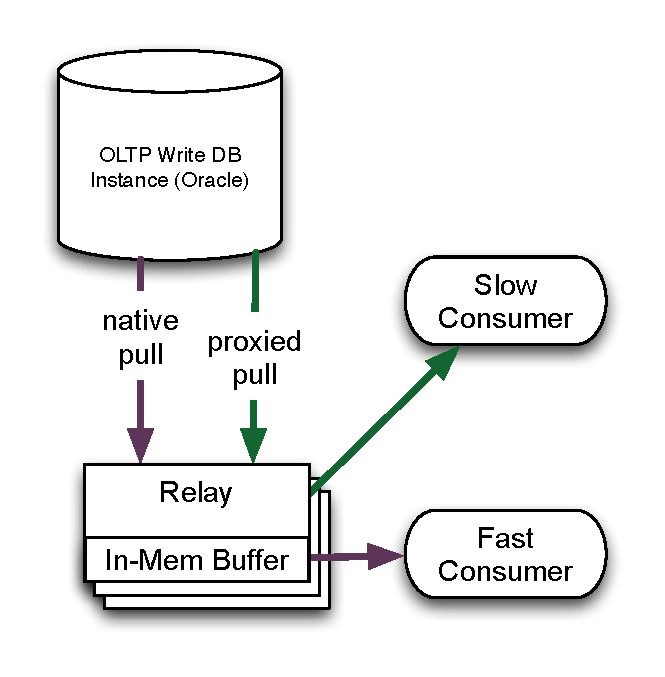
\epsfig{file=figures/databus-v1-arch.eps, scale=0.40}
\caption{LinkedIn: Databus Architecture circa 2007}
\label{fig:databus-v1-arch}
\end{figure}

\subsection{The Good}
\begin{itemize*}
\item \emph{Source Isolation}: In the original implementation of Databus, when a consumer fell too far behind, it would get proxied through to the source database. Our experience has shown that there are many reasons why clients often fall behind by a lot in unexpected ways. The most common cases happen when clients bootstrap themselves with state from data in offline systems like Hadoop, and then come online and have to catch-up a week's worth of data. Another set of cases arise due to software bugs. There have been cases where ``bad'' or unprocessable data has been written to the database or the consumer logic had bugs which made it choke on a particular event. Since the Databus framework provides in-order delivery guarantees, it retries some number of times and eventually stops. 
A third category of reasons are bursts or spikes of activity on the primary datasets, where downstream consumers which are typically provisioned for consuming the steady flow of events during normal operation, are unable to keep up with bursts of data and start falling behind. As explained in the Oracle fetcher implementation, the further the consumers fall behind, the more expensive the pull queries get, so a problem on the consumer side gets translated to a problem on the source database. When we added the Bootstrap database to the Databus architecture, we took away the capability of the consumer to impact the source database in this way. Now, catch-up queries from consumers that are very far behind are served off of the bootstrap database which is isolated and optimized for this purpose. In this way, we've managed to reduce load on the source databases enormously while being able to keep up with the client demands easily.  We routinely see clients seamlessly connecting to the bootstrap service, sometimes on a daily basis but just catching up quietly without raising any alarm bells. 
\item \emph{Common Data Format}: The original implementation of Databus used hand-written Java classes to represent the table rows, and serialized them using Java serialization. This created two problems. Firstly, everytime the table's schema was changed, someone would have to hand-edit the Java class; secondly, because the Java serialization of that object was not backwards compatible with the previous version of the object, all downstream consumers would need to get upgraded to pick up the new class definition. The workaround for this problem was to create a new view everytime the schema was changed, essentially creating one view per schema version on the database, and one copy of the event per version. As consumers evolved to picking up the new versions of the classes, the old views could be retired. In practice, consumers rarely had incentive to upgrade unless they needed the extra fields, thus the old views tended to stay around forever. The utilization of the relay buffer would worsen because each event would get serialized multiple times for each view version. In our latest changes, we moved to Avro, got rid of the multiple versions and this gave us an immediate performance win of 300\% in terms of read and write load on the source database as well as utilization of the relay buffer. 
\item \emph{Rich subscription support}: At LinkedIn we see a wide variety of consumers which are themselves partition-aware. For example, our distributed search system has many hundreds of nodes and each node only indexes a fraction of the complete data set. 
Often, different consumers want different partitioning functions or axes, and it is an organizational challenge to force everyone to agree to the same partitioning model. For example, our search engine
 uses range-based partitioning, while our relevance engine uses mod-based partitioning. Earlier, all the individual machines would pull the entire stream and filter it client-side by dropping the events that they were not interested in. When we added server-side filtering to Databus, we allowed consumers to specify their filtering function while subscribing to the sources. This has resulted in huge network savings of more than 40 times the earlier bandwidth requirements.
\end{itemize*}

\subsection{The Bad}
We haven't solved all our problems yet. There are a few open issues that we are thinking deeply about and working on. 
\begin{itemize*}
\item \emph{Oracle Fetcher performance}: Our experience has shown several factors that can negatively affect the performance of the Oracle fetcher:
\begin{itemize*}
\item Complex join views used as Databus sources as those views have to be evaluated at fetch time
\item Having large BLOBs and CLOBs as part of the row as these can incur additional disk seeks to read
\item Very high update rate can cause increase load on the SCN update job; this affects the effectiveness of the indexes on the TxLog table.
\end{itemize*}
\item \emph{Seeding the Bootstrap DB}: Seeding the Bootstrap database with large data sets from the primary store can be a challenge because of the need to extract a consistent snapshot of the data. Since stopping the writes to the primary store to seed the Bootstrap database is rarely an option, we either have to procure additional hardware to load stable backup or devise an efficient restartable algorithm that can read the data out of the primary store in small chunks while guaranteeing that no updates are going to be missed and that all transactions that happen during the seeding process are fully applied at the end. We chose to use the second approach. What our production experience has shown is that sources with complex joins and/or large BLOBs can negatively affect seeding performance. In some cases with complex joins, we have used dumps of the source tables and computed the joins offline. With such an approach, the main challenge is ensuring that the offline join produces \emph{exactly} the same results as if it was performed by the primary store, because the two table dumps may not be consistent with each other.
%%\item \emph{Bottleneck identification}: Another class of experiences that we have had during our operation of Databus at LinkedIn is with identifying bottlenecks in the pipeline. The pervasiveness of the use of Databus at LinkedIn means that it is used in a large variety of scenarios with different types of consumer processing. Whenever a performance problem is observed, we need to detect whether it is because of bottlenecks in the Databus transport tier, inefficiencies in the way the application uses Databus or an external bottleneck such as a data store that the application is writing to. The last use case is typical for large consumer clusters where we can spend significant time optimizing performance to discover that the bottleneck is caused by scalability issues in another service used by the consumer.
\end{itemize*}

